% !TEX program = pdflatex
\documentclass[12pt,a4paper]{article}

% Encoding
\usepackage[utf8]{inputenc}
%\usepackage[T1]{fontenc}
%\usepackage{lmodern}

% Math
\usepackage[fleqn]{amsmath}
\usepackage{amssymb}
\usepackage{mathtools}
% Float placement
\usepackage{float}

% Language
\usepackage[ngerman]{babel}

% Page format
\usepackage{a4wide}
\setlength{\parindent}{0pt}
\setlength{\parskip}{0.6em}

% Lists
\usepackage{enumitem}

% Graphics/links (ohne externe Bilder, damit es sicher kompiliert)
\usepackage{hyperref}
\usepackage{xcolor}

% TikZ circled numbers
\usepackage{tikz}
\newcommand*\circled[1]{\tikz[baseline=(char.base)]{
  \node[shape=circle,draw,inner sep=1.6pt] (char) {#1};}}

% Differential (wie in deiner Vorlage)
\newcommand{\dd}{\,\mathrm d}

% PDF metadata -----------------------------------
\hypersetup{
  pdfauthor={Sebastian Domaschke},
  pdftitle={FE-Grundlagen: U05 Galerkin Loesung},
  colorlinks=true,
  urlcolor=blue
}
% STYLE ==========================================

% Font family ------------------------------------
\renewcommand{\familydefault}{\sfdefault}           % sans serif as default

\begin{document}

\thispagestyle{empty}
\noindent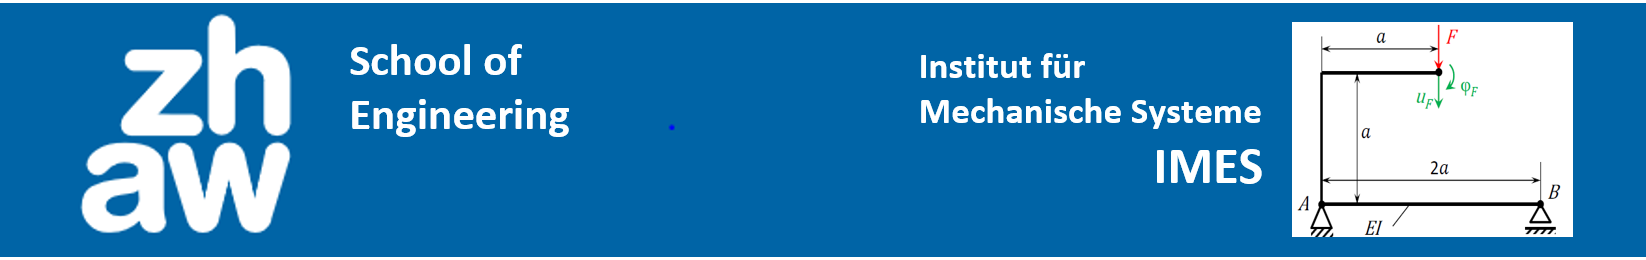
\includegraphics[width=\linewidth]{Logo.png}

\bigskip
\begin{minipage}[t]{0.55\textwidth}
  \textbf{\Huge FE-Grundlagen}\\[.4ex]
\end{minipage}
\hfill
\begin{minipage}[t]{0.42\textwidth}
  \raggedleft
  \textbf{\Huge U09 Galerkin}\\[.4ex]
  Lösung
\end{minipage}

\noindent\rule{\linewidth}{1.8pt}



\section*{Einleitung}
In dieser Übung bestimmen wir mit der Galerkin-Methode Näherungslösungen für das Verschiebungsfeld $u(x)$ eines eindimensionalen Stabs.

\section*{Stab mit Linienlast}
Der Stab der Länge~$L$ ist wie abgebildet rechtsseitig eingespannt mit einer vorgegegebenen Verschiebung~$\bar{u}_L \neq 0$.
Sowohl Querschnitt~$A$ als auch E-Modul~$E$ seien konstant.
Über der Stab\-länge verteilt wirkt die axiale Linienlast $n(x)=\nu\,A\,x^2$ und zusätzlich links die Zugspannung~$\bar{t}_0$.
Die schwache Form des Gleichgewichts ist in~\eqref{eqn:Weak} gegeben.

\bigskip

\begin{minipage}[t]{.43\textwidth}
  \subsubsection*{System}
  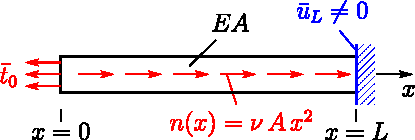
\includegraphics[]{truss}
\end{minipage}
\subsubsection*{Schwache Form des Gleichgewichts}
\begin{equation}\tag{$*$}\label{eqn:Weak}
\begin{split}
0 =\;& -\int_0^L g'(x)\,EA\,u'(x)\,\dd x
\;-\; g(0)\,A\,\bar t_0
\;+\;\int_0^L g(x)\,\nu A\,x^2\,\dd x\\
&\qquad \forall g \ \text{(verträglich)}.
\end{split}
\end{equation}

\medskip
Wichtig: Die essentielle Randbedingung ist $u(L)=\bar u_L$.
Darum müssen die \emph{verträglichen} Gewichtungsfunktionen erfüllen:
\[
g(L)=0.
\]

%%%%%%%%%%%%%%%%%%%%%%%%%%%%%%%%%%%%%%%%%%%%%%%%%%%%%%%%%%%%%%%%%%%%%%%%%%%%%%
\subsubsection*{Teil I: Näherungslösungen nach Galerkin (3 Varianten)}
%%%%%%%%%%%%%%%%%%%%%%%%%%%%%%%%%%%%%%%%%%%%%%%%%%%%%%%%%%%%%%%%%%%%%%%%%%%%%%

\paragraph{Teil 1a) Linearer Ansatz}

\begin{enumerate}[label=\protect\circled{\arabic*}]
\item \textbf{Ansatzfunktion}
\begin{equation}\label{eqn:Trial}
u(x)=c_0+c_1x.
\end{equation}

\item \textbf{Passende Gewichtungsfunktion (Galerkin)}\\
Galerkin: Testfunktionen aus demselben Ansatzraum:
\begin{equation}\label{eqn:Test}
g_u(x)=\delta c_0+\delta c_1x.
\end{equation}

\item \textbf{Randbedingung in den Ansatz einsetzen}\\
\[
u(L)=c_0+c_1L=\bar u_L
\quad\Rightarrow\quad
c_0=\bar u_L-c_1L.
\]
Also
\begin{equation}\label{eqn:TrialSimple}
u(x)=\bar u_L+c_1(x-L).
\end{equation}

\item \textbf{Verträglichkeit der Gewichtungsfunktion}\\
Weil $g(L)=0$ gelten muss:
\[
g_u(L)=\delta c_0+\delta c_1L=0
\quad\Rightarrow\quad
\delta c_0=-\delta c_1L.
\]
Damit
\begin{equation}\label{eqn:TestSimple}
g_u(x)=\delta c_1(x-L).
\end{equation}
\medskip
\item \textbf{Ableiten}
\begin{align}
u'(x) &= c_1, \label{eqn:TrialPrime}\\
g'(x) &= \delta c_1. \label{eqn:TestPrime}
\end{align}

\item \textbf{In die schwache Form einsetzen, $c_1$ bestimmen}\\
Setze $u'(x)=c_1$, $g'(x)=\delta c_1$, $g(0)=-\delta c_1L$ und $g(x)=\delta c_1(x-L)$ in \eqref{eqn:Weak}:
\begin{align*}
0
&= -\int_0^L \delta c_1\cdot EA\cdot c_1\,\dd x
\;-\;(-\delta c_1L)\,A\,\bar t_0
\;+\;\int_0^L \delta c_1(x-L)\,\nu A\,x^2\,\dd x.
\end{align*}
Die Terme einzeln:
\[
\,-\int_0^L \delta c_1\,EA c_1\,\dd x = -\delta c_1\,EA c_1 L,
\qquad
\,-(-\delta c_1L)A\bar t_0 = +\delta c_1LA\bar t_0.
\]
Für die Linienlast:
\begin{align*}
\int_0^L \delta c_1(x-L)\,\nu A\,x^2\,\dd x
&=\delta c_1\,\nu A\int_0^L (x^3-Lx^2)\,\dd x\\
&=\delta c_1\nu A\left[\frac{x^4}{4}-L\frac{x^3}{3}\right]_0^L\\
&=\delta c_1\nu A\left(\frac{L^4}{4}-\frac{L^4}{3}\right)
=-\delta c_1\nu A\frac{L^4}{12}.
\end{align*}
Zusammen:
\[
0=-\delta c_1\,EA c_1 L +\delta c_1LA\bar t_0-\delta c_1\,\nu A\frac{L^4}{12}.
\]
\[
0=\delta c_1\underbrace{\Bigl(-\,EA c_1 L +LA\bar t_0-\,\nu A\frac{L^4}{12}\Bigr)}_{=0}.
\]
Da $\delta c_1$ frei wählbar ist (und nicht identisch $0$), muss der Term in der Klammer gleich 0 sein. Zudem lässt sich $AL$ kürzen. Es folgt.:
\[
Ec_1=\bar t_0-\nu\frac{L^3}{12}
\quad\Rightarrow\quad
\boxed{c_1=\frac{\bar t_0-\nu L^3/12}{E}}.
\]
Damit:
\[
\boxed{
u^{(1)}(x)=\bar u_L+\frac{\bar t_0-\nu L^3/12}{E}\,(x-L)
}.
\]
\end{enumerate}

\paragraph{Teil 1b) Quadratischer Ansatz}
Ansatz:
\[
u(x)=c_0+c_1x+c_2x^2.
\]
Randbedingung $u(L)=\bar u_L$:
\[
c_0=\bar u_L-c_1L-c_2L^2.
\]
Praktische Form:
\[
u(x)=\bar u_L+c_1(x-L)+c_2(x^2-L^2).
\]
Wähle gemäss Galerkin Testfunktionen aus dem selben Ansatzraum (konsistent zum Ansatz: $\delta c_1$ zum linearen, $\delta c_2$ zum quadratischen Term):
\[
g_u(x)=\delta c_1(x-L)+\delta c_2(x^2-L^2).
\]
Ableitungen:
\[
u'(x)=c_1+2c_2x.
\]

\medskip
\textbf{Schwache Form auswerten (Schritt für Schritt):} Setze
\[
u'(x)=c_1+2c_2x,\qquad
g_u'(x)=\delta c_1+2\delta c_2x,\qquad
g_u(0)=-\delta c_1L-\delta c_2L^2.
\]

Einsetzen in \eqref{eqn:Weak} ergibt (nach Kürzen von $A$):
\[
0=-E\!\int_0^L(\delta c_1+2\delta c_2x)(c_1+2c_2x)\,\dd x
 -\,g_u(0)\,\bar t_0
 +\,\nu\!\int_0^L(\delta c_1(x-L)+\delta c_2(x^2-L^2))x^2\,\dd x.
\]

\textbf{Steifigkeitsterm:}
\[
-E\!\int_0^L(\delta c_1+2\delta c_2x)(c_1+2c_2x)\,\dd x
=-E\!\int_0^L\!\Bigl(\delta c_1c_1+2\delta c_1c_2x+2\delta c_2c_1x+4\delta c_2c_2x^2\Bigr)\dd x
\]
\[
=-E\Bigl(\delta c_1c_1L+\delta c_1c_2L^2+\delta c_2c_1L^2+\frac{4}{3}\delta c_2c_2L^3\Bigr).
\]

\textbf{Randterm:}
\[
-g_u(0)\bar t_0=(\delta c_1L+\delta c_2L^2)\bar t_0.
\]

\textbf{Lastterm:}
\[
\nu\!\int_0^L(\delta c_1(x-L)+\delta c_2(x^2-L^2))x^2\,\dd x
=\nu\!\int_0^L\!\Bigl(\delta c_1(x^3-Lx^2)+\delta c_2(x^4-L^2x^2)\Bigr)\dd x
\]
\[
=\nu\Bigl(\delta c_1\bigl(\tfrac{L^4}{4}-\tfrac{L^4}{3}\bigr)
  +\delta c_2\bigl(\tfrac{L^5}{5}-\tfrac{L^5}{3}\bigr)\Bigr)
=-\nu\Bigl(\delta c_1\frac{L^4}{12}+\delta c_2\frac{2}{15}L^5\Bigr).
\]

Zusammen:
\[
0=\delta c_1\Bigl(-E(c_1L+c_2L^2)+L\bar t_0-\nu\frac{L^4}{12}\Bigr)
\;+\;\delta c_2\Bigl(-E\!\left(c_1L^2+\frac{4}{3}c_2L^3\right)+L^2\bar t_0-\nu\frac{2}{15}L^5\Bigr).
\]

Da $\delta c_1$ und $\delta c_2$ unabhängig sind, folgen die zwei Gleichungen (jeweils durch $L$ bzw.\ $L^2$ gekürzt):
\[
E(c_1+Lc_2)=\bar t_0-\nu\frac{L^3}{12},\qquad
E\!\left(c_1+\frac{4}{3}Lc_2\right)=\bar t_0-\nu\frac{2}{15}L^3.
\]

\medskip
\textbf{Lösen:}\\
Subtraktion liefert
\[
E\left(\frac{1}{3}Lc_2\right)
=-\nu\left(\frac{2}{15}-\frac{1}{12}\right)L^3
=-\nu\frac{1}{20}L^3
\quad\Rightarrow\quad
\boxed{c_2=-\frac{3\nu L^2}{20E}}.
\]
In die erste Gleichung:
\[
E c_1=\bar t_0+\nu L^3\left(\frac{3}{20}-\frac{1}{12}\right)
=\bar t_0+\nu\frac{L^3}{15}
\quad\Rightarrow\quad
\boxed{c_1=\frac{\bar t_0+\nu L^3/15}{E}}.
\]
Damit:
\[
\boxed{
u^{(2)}(x)=\bar u_L+\frac{\bar t_0+\nu L^3/15}{E}(x-L)
-\frac{3\nu L^2}{20E}(x^2-L^2)
}.
\]

\paragraph{Teil 1c) Trigonometrischer Ansatz}

\[
u(x)=a_0+a_1\sin\!\left(\frac{x}{L}\right).
\]
Randbedingung $u(L)=\bar u_L$:
\[
a_0=\bar u_L-a_1\sin(1).
\]
Also
\[
u(x)=\bar u_L+a_1\Bigl(\sin\!\left(\tfrac{x}{L}\right)-\sin(1)\Bigr).
\]
Wähle eine Galerkin-Testfunktion vom selben Typ, mit anderen Worten aus dem selben Ansatzraum:
\[
g_u(x)=\delta a_1\Bigl(\sin\!\left(\tfrac{x}{L}\right)-\sin(1)\Bigr).
\]
Ableitungen:
\[
g_u'(x)=\frac{\delta a_1}{L}\cos\!\left(\tfrac{x}{L}\right),
\qquad
u'(x)=\frac{a_1}{L}\cos\!\left(\tfrac{x}{L}\right).
\]

Einsetzen in \eqref{eqn:Weak}:
\[
0=-\int_0^L g_u'(x)\,EA\,u'(x)\,\dd x
-g_u(0)\,A\,\bar t_0
+\int_0^L g_u(x)\,\nu A\,x^2\,\dd x.
\]
Alle Terme sind proportional zu $A$, deshalb können wir durch $A$ teilen (wieder: $A$ kürzt sich heraus).
Die drei Beiträge:

\textbf{(i)} Steifigkeitsterm:

\[
\Rightarrow\quad
-\int_0^L g_u' E u'\,\dd x
=-E a_1\delta a_1\int_0^L \frac{1}{L^2}\cos^2\!\left(\tfrac{x}{L}\right)\dd x.
\]

Mit dem Tipp:
\[
\int \cos^2\!\left(\tfrac{x}{L}\right)\dd x=\frac{x}{2}+\frac{L}{4}\sin\!\left(\tfrac{2x}{L}\right)+C
\]
\[
\Rightarrow\quad
\int_0^L \cos^2\!\left(\tfrac{x}{L}\right)\dd x
=\left[\frac{x}{2}+\frac{L}{4}\sin\!\left(\tfrac{2x}{L}\right)\right]_0^L
=\frac{L}{2}+\frac{L}{4}\sin(2).
\]

Damit:
\[
-\int_0^L g_u' E u'\,\dd x
=-E a_1\delta a_1\frac{1}{L^2}\left(\frac{L}{2}+\frac{L}{4}\sin(2)\right)
=-E a_1\delta a_1\frac{1}{L}\left(\frac12+\frac{\sin(2)}{4}\right).
\]

\textbf{(ii)} Randterm: $g_u(0)=-\delta a_1\sin(1)$, daher
\[
-g_u(0)\bar t_0=+\delta a_1\sin(1)\,\bar t_0.
\]

\textbf{(iii)} Lastterm:

\[
\int_0^L g_u(x)\,\nu x^2\,\dd x
=\delta a_1\nu\!\int_0^L x^2\sin\!\left(\tfrac{x}{L}\right)\dd x
-\delta a_1\nu\sin(1)\!\int_0^L x^2\,\dd x.
\]

Mit dem Tipp:
\[
\int x^2\sin\!\left(\tfrac{x}{L}\right)\dd x
=-Lx^2\cos\!\left(\tfrac{x}{L}\right)
+2L^2x\sin\!\left(\tfrac{x}{L}\right)
+2L^3\cos\!\left(\tfrac{x}{L}\right)+C.
\]

Einsetzen der Grenzen:
\[
\int_0^L x^2\sin\!\left(\tfrac{x}{L}\right)\dd x
=\Bigl[-Lx^2\cos\!\left(\tfrac{x}{L}\right)
+2L^2x\sin\!\left(\tfrac{x}{L}\right)
+2L^3\cos\!\left(\tfrac{x}{L}\right)\Bigr]_0^L
=L^3\bigl(\cos(1)+2\sin(1)-2\bigr).
\]

Außerdem:
\[
\int_0^L x^2\,\dd x=\frac{L^3}{3}.
\]

Damit:
\[
\int_0^L g_u(x)\,\nu x^2\,\dd x
=\delta a_1\nu L^3\Bigl(\cos(1)+2\sin(1)-2-\frac{1}{3}\sin(1)\Bigr)
=\delta a_1\nu L^3\left(\cos(1)+\frac{5}{3}\sin(1)-2\right).
\]

Somit:
\[
0=\delta a_1\Biggl(
-E a_1\frac{1}{L}\left(\frac12+\frac{\sin(2)}{4}\right)
+\sin(1)\bar t_0
+\nu L^3\left(\cos(1)+\frac{5}{3}\sin(1)-2\right)\Biggr).
\]
Auflösen:
\[
\boxed{
a_1=
\frac{L}{E\left(\frac12+\frac{\sin(2)}{4}\right)}
\left[
\sin(1)\bar t_0+\nu L^3\left(\cos(1)+\frac{5}{3}\sin(1)-2\right)
\right]
}.
\]
Damit:
\[
\boxed{
u^{(\sin)}(x)=\bar u_L+a_1\Bigl(\sin\!\left(\tfrac{x}{L}\right)-\sin(1)\Bigr)
}.
\]

%%%%%%%%%%%%%%%%%%%%%%%%%%%%%%%%%%%%%%%%%%%%%%%%%%%%%%%%%%%%%%%%%%%%%%%%%%%%%%
\subsubsection*{Teil II: Vergleich (Näherungen vs. analytisch)}
%%%%%%%%%%%%%%%%%%%%%%%%%%%%%%%%%%%%%%%%%%%%%%%%%%%%%%%%%%%%%%%%%%%%%%%%%%%%%%

Die analytische Lösung zu \eqref{eqn:Weak} ist gegeben als
\begin{equation}\label{eqn:Solution}
\hat{u}(x)=\bar u_L+\frac{\bar t_0}{E}(x-L)-\frac{\nu}{12E}(x^4-L^4).
\end{equation}
Hinweis: Da in \eqref{eqn:Weak} überall ein Faktor $A$ vorkommt, kürzt sich $A$ in der Differentialgleichung und in der schwachen Form heraus.
Darum ist es konsistent, dass \eqref{eqn:Solution} nicht von $A$ abhängt.

\paragraph{Wie gut passen Ihre Näherungslösungen aus Teil 1a)–1c) zur analytischen Lösung?}
Mit den vorgegebenen Werten:
\[
E=10^5,\quad L=2,\quad \nu=1,\quad \bar u_L=0,\quad \bar t_0=10.
\]

\textbf{Analytisch:}
\[
\hat u(x)=\frac{10}{10^5}(x-2)-\frac{1}{12\cdot 10^5}(x^4-16),
\qquad
\hat\sigma(x)=E\hat u'(x)=10-\frac{x^3}{3}.
\]

\textbf{Linear (Teil 1a):}
\[
c_1=9.3333\cdot 10^{-5},\qquad
u^{(1)}(x)=c_1(x-2),\qquad
\sigma^{(1)}(x)=9.3333.
\]

\textbf{Quadratisch (Teil 1b):}
\[
c_1=1.05333\cdot 10^{-4},\qquad
c_2=-6.0\cdot 10^{-6},
\]
\[
u^{(2)}(x)=c_1(x-2)+c_2(x^2-4),\qquad
\sigma^{(2)}(x)=10.5333-1.2x.
\]


\textbf{Trigonometrisch (Teil 1c):}
\[
a_1\approx 2.18795\cdot 10^{-4},\qquad
u^{(\sin)}(x)=a_1\Bigl(\sin\!\left(\tfrac{x}{2}\right)-\sin(1)\Bigr),
\]
\[
\sigma^{(\sin)}(x)=10^5\frac{a_1}{2}\cos\!\left(\tfrac{x}{2}\right).
\]

\newpage
\textbf{Grafischer Vergleich der Näherungen mit der analytischen Lösung}

\begin{figure}[H]
  \centering
  \includegraphics[width=0.75\linewidth]{plots_u.png}
  \caption{Verschiebung $u(x)$: analytisch vs. Näherungen (linear, quadratisch, trigonometrisch).}
\end{figure}

\begin{figure}[H]
  \centering
  \includegraphics[width=0.75\linewidth]{plots_sigma.png}
  \caption{Spannung $\sigma(x)$: analytisch vs. Näherungen (linear, quadratisch, trigonometrisch).}
\end{figure}

\paragraph{Diskussion der Ergebnisse}
Die Verschiebungen stimmen in allen drei Varianten sehr gut mit der analytischen Lösung überein. Am besten passt der quadratische Ansatz.

Deutlicher sind die Unterschiede in der Spannung, die von den Ableitungen der Verschiebungen abhängen: 
der lineare Ansatz liefert eine konstante Spannung, der quadratische eine lineare, während die exakte Spannung kubisch ist. 
Damit verbessert der quadratische Ansatz die Spannung sichtbar, der trigonometrische Ansatz liegt ebenfalls näher an der exakten Krümmung, ohne sie exakt zu treffen.

%%%%%%%%%%%%%%%%%%%%%%%%%%%%%%%%%%%%%%%%%%%%%%%%%%%%%%%%%%%%%%%%%%%%%%%%%%%%%%
\subsubsection*{Teil III: Theoretische Diskussion}
%%%%%%%%%%%%%%%%%%%%%%%%%%%%%%%%%%%%%%%%%%%%%%%%%%%%%%%%%%%%%%%%%%%%%%%%%%%%%%

\begin{enumerate}[label={},leftmargin=*]
\item[\circled{1}] \textbf{Durch welche Massnahmen könnte die Näherung verbessert werden?}\\
Ansatzraum erweitern (mehr Freiheitsgrade), oder stückweise Ansatzfunktionen (klassische FEM), also $p$-, $h$- oder $hp$-Verfeinerung.

\item[\circled{2}] \textbf{Wie konkret vorgehen?}\\
Entweder
\begin{itemize}
  \item in FEM-Software Element mit  höherem Polynomgrad wählen (p-Verfeinerung) oder
  \item Stab in meherere Elemente zerlegen, also ein feineres Netz nutzen (h-Verfeinerung).
\end{itemize}

\item[\circled{3}] \textbf{Für welche Gewichtungsfunktionen $g$ erfüllt $\hat u$ die schwache Form?}\\
Für alle genügend glatten, verträglichen Gewichtungsfunktionen, die die essentielle RB respektieren:
\[
\boxed{g \text{ ist stetig, stückweise differenzierbar und erfüllt } g(L)=0.}
\]

\item[\circled{4}] \textbf{Für welche Gewichtungsfunktionen $g_u$ erfüllen die Näherungen aus Teil I die schwache Form?}\\
Jeweils nur für $g_u$ aus dem gewählten Testraum:
\[
\boxed{\text{linear: } g_u(x)=\alpha\,(x-L)},
\qquad
\boxed{\text{quadratisch: } g_u(x)=\alpha\,(x-L)+\beta\,(x^2-L^2)},
\]
\[
\boxed{\text{trig.: } g_u(x)=\alpha\left(\sin\!\left(\tfrac{x}{L}\right)-\sin(1)\right)}.
\]

\end{enumerate}

\end{document}